%!TEX root = ./intern_report.tex

\newpage
\subsection{Hillnet: An Experimental Attempt at Utilizing ML for Hill Climbing}

\paragraph{}
After successfully demonstrating indoor-Trailnet built from scratch, trained and deployed with my pipeline, our supervisor Nick described about his idea of experimenting with a algorithm to climb hills while avoiding obstacles using computer vision. We were asked to come up with a system where two different types of inputs are merged: scaler inputs representing the direction of the slope and the RGB image input from a camera to output a velocity command to control the motor controller. Trailnet, which itself was based on resnet-18 was chosen to be modified to build such a neural network.

\subsubsection{Preprocessing IMU and Velocity Data}

\paragraph{}
The LORD Microstrain IMU sends its data through serial to its ROS package, which publishes the IMU readings in two types: as a quaternion and set of cartesian x,y,z vector components of perceived acceleration. I decided to use the vector components to calculate the magnitude and direction of the gravity vector projected on the horizontal plane of the robot. Direction $\theta \in [-\pi, \pi]$ was measured with respect to the heading direction and then converted to $[0, 1]$ range using the sigmoid function to match the range of the other normalized inputs. I chose to output the angular velocity as a float $\in [0,1]$ using a sigmoid output node (in classification approach) and scale it to the necessary angular Velocity.

\begin{align*}
    x, y, z   &= \text{Magnitude of the cartesian components of perceived acceleration. x: forward, z: vertical} \\
    r, \theta &= \text{polar components of the acceleration vector projected on the horizontal plane of robot} \\
    r_{in}, theta_{in}     &= \text{processed values given as input to the network}
\end{align*}

\begin{align*}
    r &= \sqrt{x^2 + y^2} \\
    r_{in} &= \tfrac{r}{g} & \text{normalized by the maximum: g} \\
    \theta &= \arctan({\tfrac{y}{x}})     &  \theta \in [-\pi,\pi] \\
    \theta_{in} &= \text{sigmoid}(\theta) &  \theta_{in} \in [0,1]
\end{align*}


\newpage
\subsubsection{Data Collection}

\paragraph{}
As per the instructions of our supervisor, Uvindu collected data in the slopes around CSIRO campus during the last few weeks of the internship. He placed the robot on the bottom of the hill and drove the robot following the steepest ascent. When he faced an obstacle, he went around the obstacle and continued to follow the steepest ascent. Image streams from the camera, IMU data and the odometry reading from the motor encoders were recorded in ROSbags.

% Image: Data Collect
\begin{figure}[H]
    \centering
    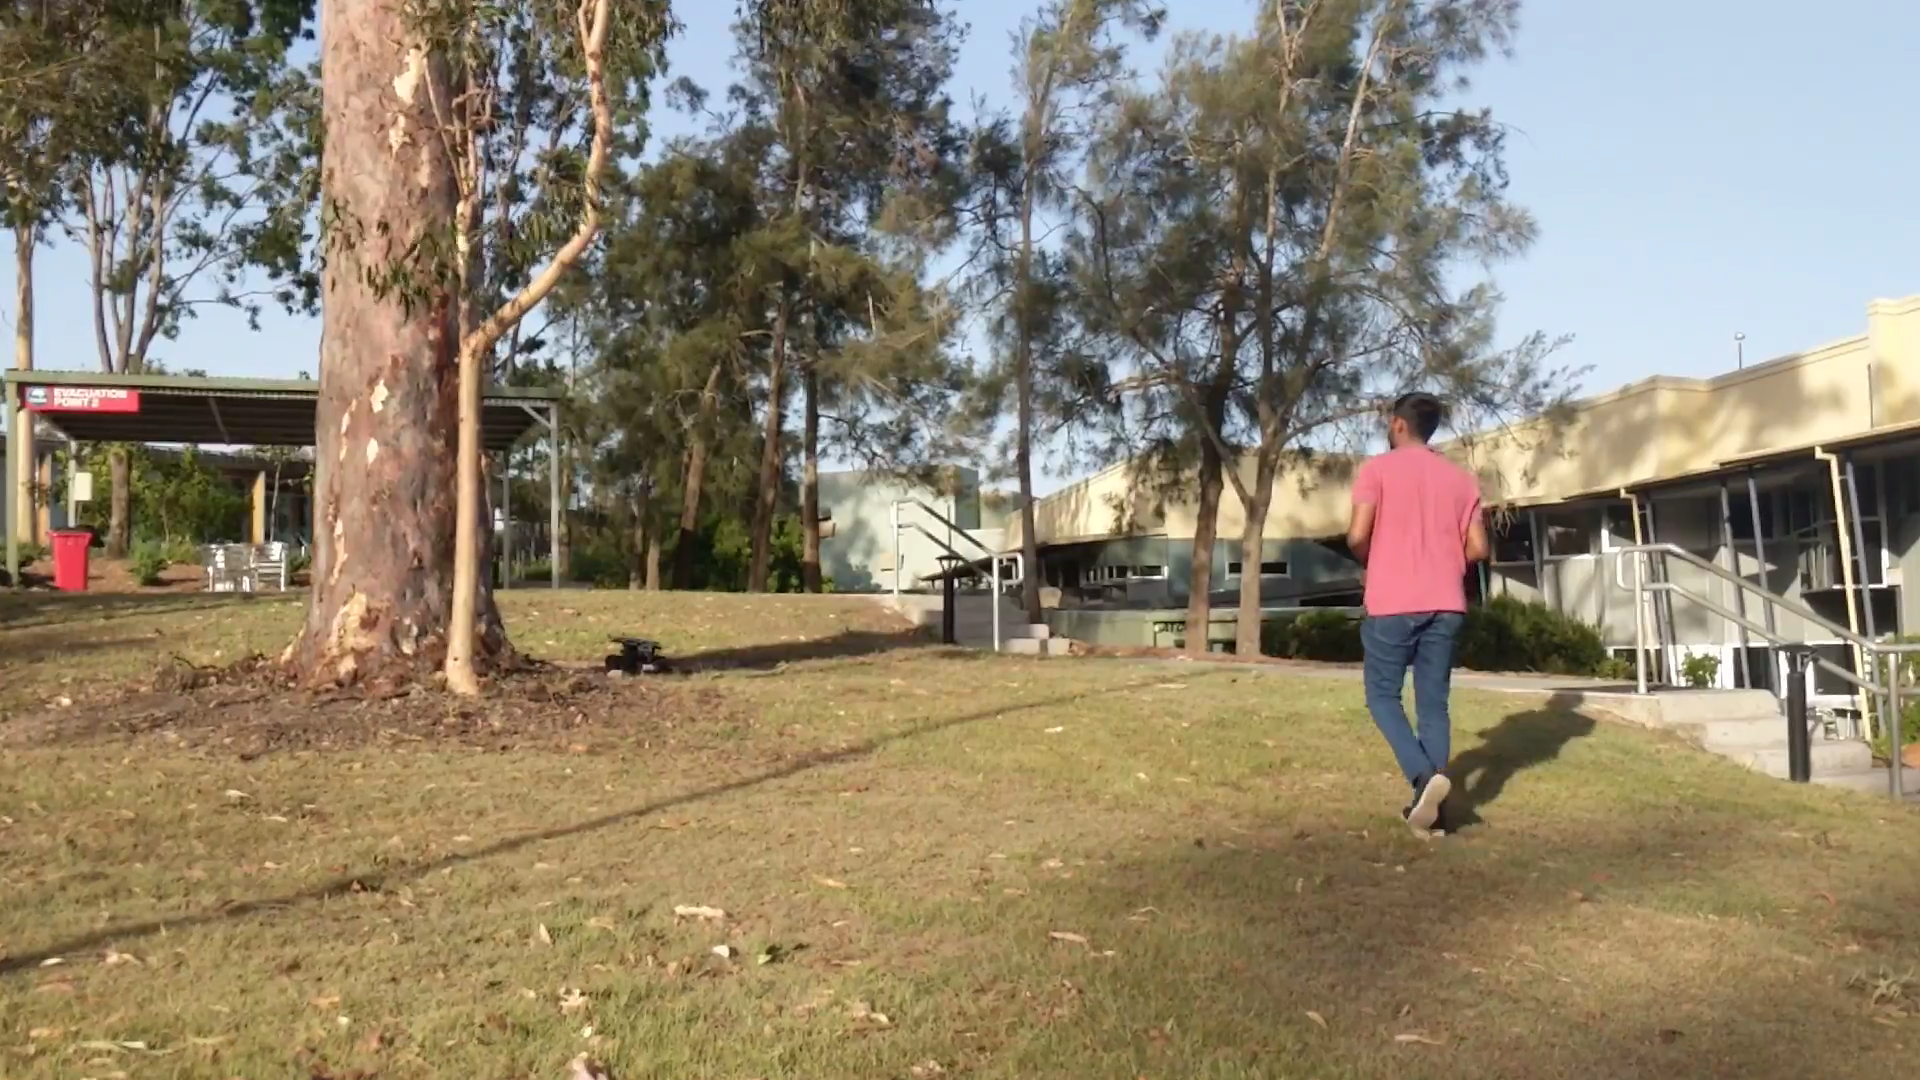
\includegraphics
        [width=8cm]
        {figures/hillnet_data_collect.png}
    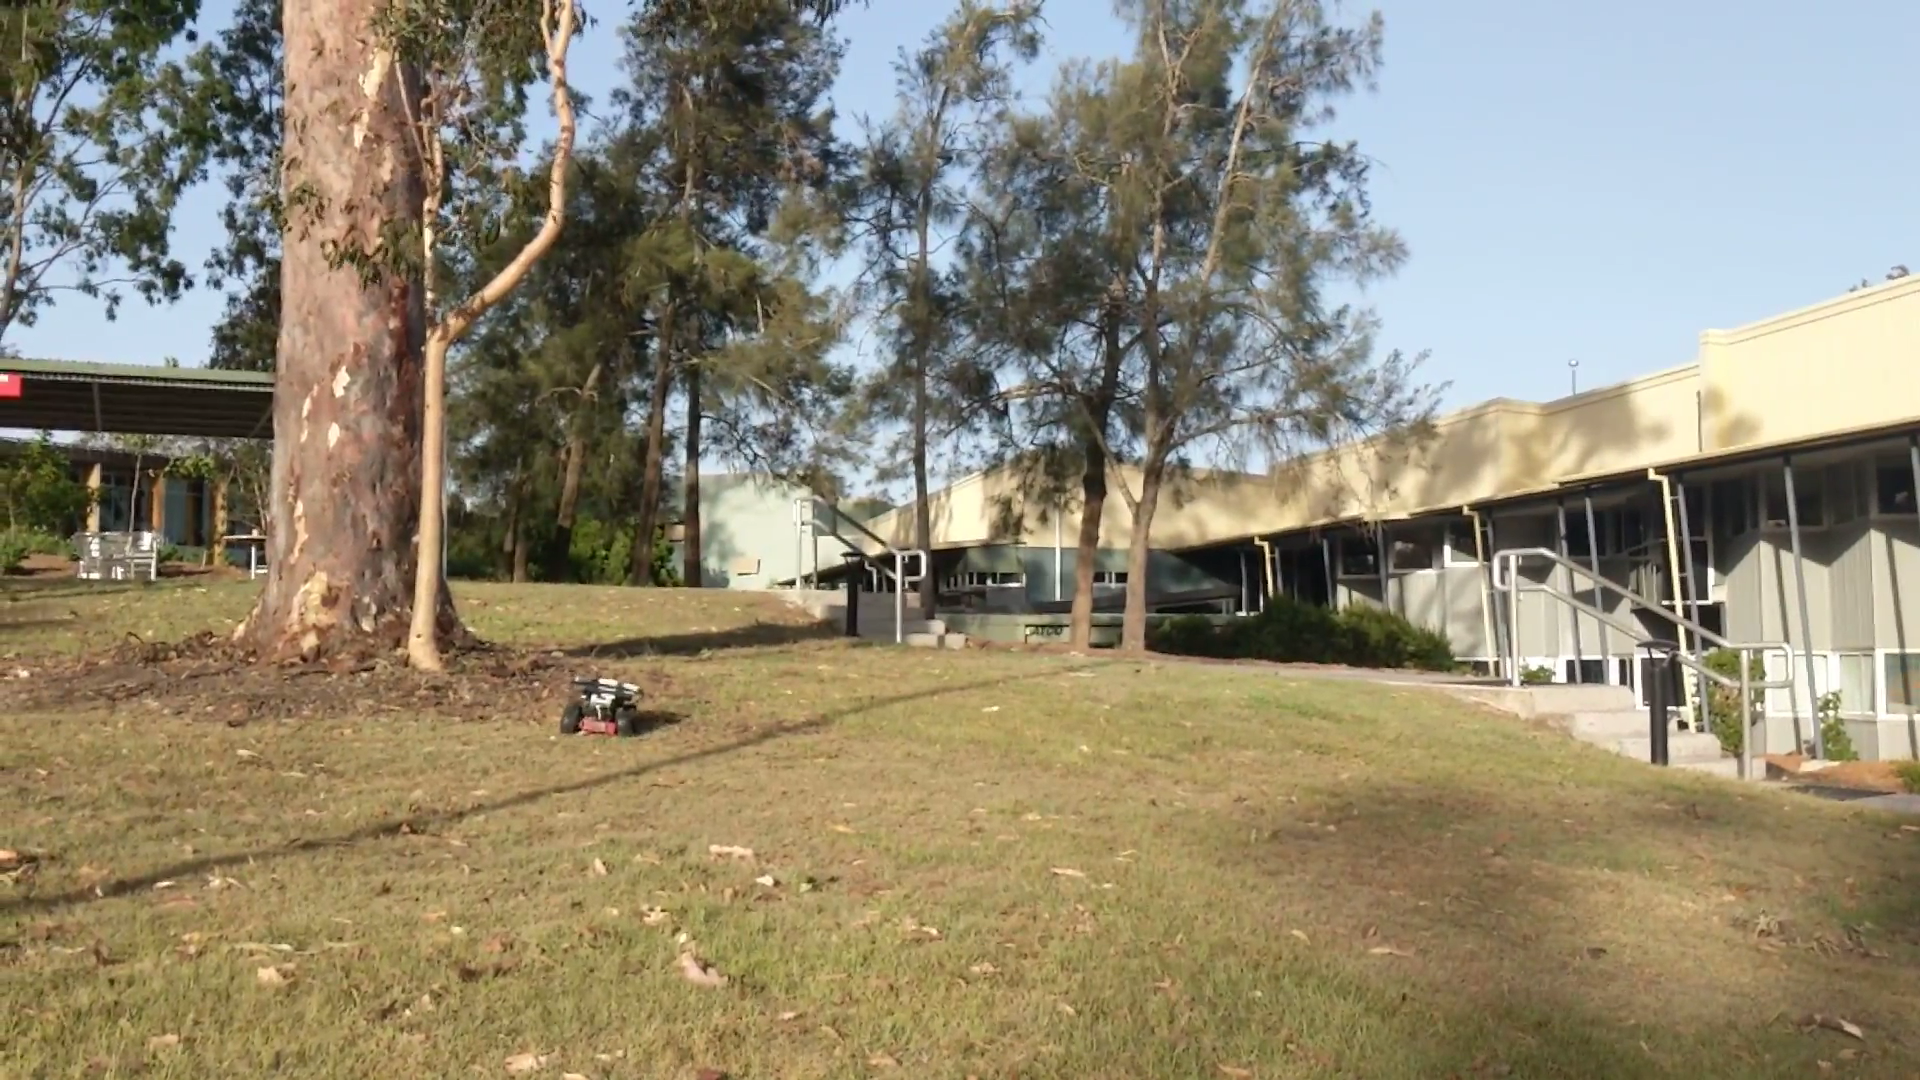
\includegraphics
        [width=8cm]
        {figures/hillnet_data_collect_2.png}
    \caption{Data Collection to Train Hillnet}\vspace{-4mm}
\end{figure}

\subsubsection{Merging Scaler and Image Inputs}

\paragraph{}
For this task, it was necessary to decide how the two types of inputs: scaler and image are combined in the neural network. Our supervisor proposed a method, where the IMU values are concatenated to the flattened output of the convolution layers, followed by few fully connected layers. The inspiration for this idea comes from the insight that deeper layers of a deep neural network identify higher level features and therefore the flattened average pooling output of the CNN should be containing information about by how much should the robot turn to avoid the obstacle. Therefore, concatenating the IMU inputs, which also tell by how much the robot should turn to follow the hill and following it with few fully connected layers might result in the network learning an OR operation between two inputs. 

\paragraph{}
However, a research paper on merging these kind of inputs ~\cite{hand_eye} proposed an alternative method, where the scaler inputs are broadcasted into a matrix with the right size, processed by few fully connected layers and added elementwise to the output of an intermediate layer in the CNN. The insight behind this is the fact that the output of the fully connected layers might act like a mask on the image, effectively clouding and directing the decision process of the CNN. After some consideration and experimentation, we decided to follow our supervisor's method since it was more suitable for our task.


% Image: Merge Inputs
\begin{figure}[H]
    \centering
    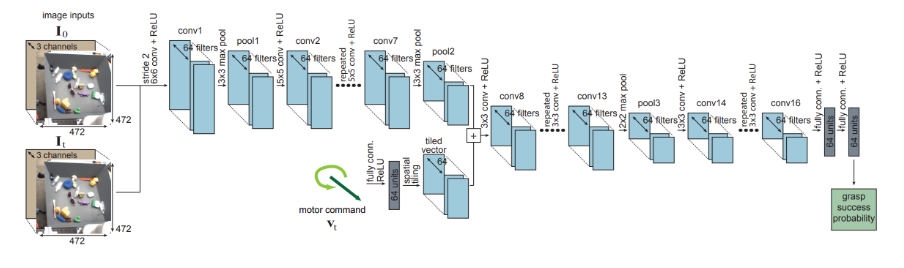
\includegraphics
        [width=16cm]
        {figures/merge_inputs.PNG}
    \caption{Merging by Broadcast and Add Elementwise as a Mask}\vspace{-4mm}
    
\end{figure}

\subsubsection{Regression Approach}

\paragraph{}
Next we brainstormed on how to post-process the output of the network to steer the robot. During the discussion, our supervisor first suggested to use the regression approach. That is, to build a network with a single output node that has no activation function, so the output value can be directly used as the angular velocity command to steer the robot. This is quite straightforward to build, train and test. The neural network can be trained with IMU and Image data and output as the angular velocity from odometry reading when driven by remote control during data collection.

% Image: Regress Architecture
\begin{figure}[H]
    \centering
    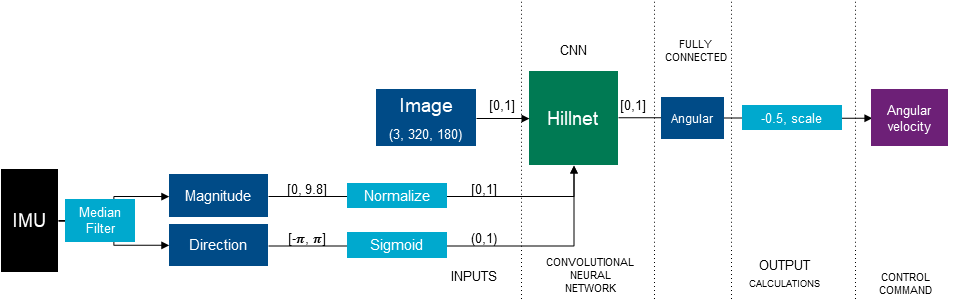
\includegraphics
        [width=16cm]
        {figures/hillnet_regress.PNG}
    \caption{Hillnet Regression Architecture}\vspace{-4mm}
    
\end{figure}

\subsubsection{Classification Approach}

\paragraph{}
During that discussion, I suggested trying a classification approach similar to that of trailnet. First advantage was the ability to fine tune the output by adjusting the constants. With regression, either it works or not. But with classification, we could fine tune it to work as we wish. Then, the effect of human error introduced in collecting data can be made insignificant by quantizing the angular velocity into classes: left, center and right. 

% Image: Classify Architecture
\begin{figure}[H]
    \centering
    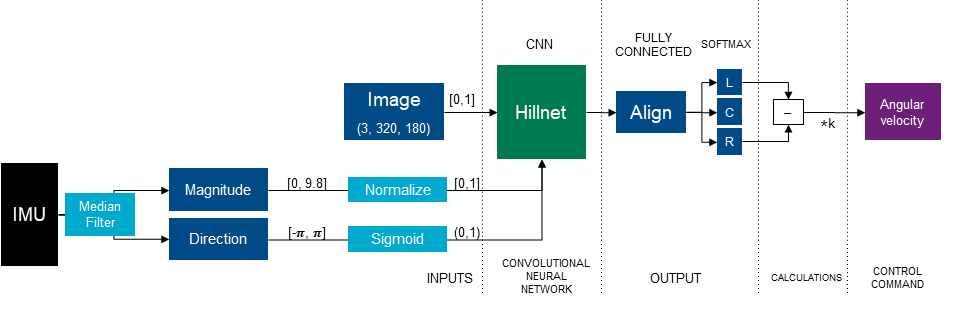
\includegraphics
        [width=16cm]
        {figures/hillnet_classify.PNG}
    \caption{Hillnet Classification Architecture}\vspace{-4mm}
    
\end{figure}

\paragraph{}
Next, I proposed a scheme of augmenting data to effectively triple the amount of collected training data. That is, first we record image streams from all three cameras. Then, in the input pipeline, I made changes to add +30\degree and -30\degree to the IMU angle and use it as datapoints along with the image streams from left and right cameras respectively. This would train the network to NOT turn away from the steepest slope, unless an obstacle is encountered, I argued. Our supervisor accepted the idea and asked me to work on both classification and regression in parallel to compare their merits. 



\subsubsection{Problems Faced and Solutions}

\paragraph{}
First problem we faced was the human errors in data collection. Since the hills had a small slope, Uvindu had difficulty in visually identifying the highest-slope direction and steering the robot towards it. When we analysed the collected data using the visualization techniques, we found there was a steady state error by up to 5\degree-10\degree. We tried collecting more data with a couple of days remaining to end the internship.

\paragraph{}
Another anomaly I observed from the visualization was the fact the IMU input had a high variance (noise). This was due to facts the slope was gentle (high percentage error) and the spring loaded suspension system of Wallie was causing it to wobble, introducing low frequency vibrations. This was critical, since our neural network does not remember nor correlate with the past inputs, but considers only the current inputs to give instantaneous outputs. Such a noisy input will prevent the training process from converging to a global maxima. Hence I suggested mounting the IMU at an angle to reduce the percentage error. After experimenting with mean and median filters of various lengths, I implemented a median filter of length 50 to smoothen the noise.

\paragraph{}
On the last few days of the internship, while debugging the network, I accidentally noticed that our collected dataset had an unhealthy disparity. That is, only 0.15\% data accounted for avoiding obstacles, while the rest 99.85\% accounted for climbing following the steepest hill. This is a classic problem in data science where the neural network simply learns to suggest "go forward" and be right 99.85\% of the time! I had discussed a similar potential problem with the supervisor at the beginning of the project, where I raised concerns that "we are not showing the robot which input-output combinations are wrong. we are showing only what is right". Our supervisor assured that "the robot will learn what is wrong, when you turn the robot to face the hill after avoiding an obstacle". However, the percentage of that kind of data was dwarfed by the "straight climbing" data in the dataset. I discussed this with Micheal and our supervisor and started implementing my idea of artificially boosting the frequency of "avoiding obstacle" data in the input pipeline.

\paragraph{}
However, we were running out of time by the end of the internship to try all possible ideas and experiment with all the possibilities. I stayed for multiple days overnight at office to try and finish as much as possible, but we couldn't try everything within that short time. Spending most of our time on building and debugging the robot platform could be one of the reasons for our time being limited for exploring new ideas with Hillnet. However, we realized that this is quite common in experimental field robotics, where scientists get to spend most of the time struggling with the hardware issues. 